%% VoI-Search WSDM 2027 camera-ready working revision
%% Build: latexmk -pdf main.tex
%% xcolor is loaded by acmart, so the table option must be passed ahead of it
\PassOptionsToPackage{table}{xcolor}
\documentclass[sigconf,balance=false]{acmart}

\usepackage{tikz}
\usetikzlibrary{arrows.meta,positioning,shapes.geometric,fit,calc,backgrounds}
\usepackage{array}
\usepackage{multirow}
\usepackage{enumitem}
\usepackage{balance}
\usepackage{needspace}
\usepackage[ruled,vlined,linesnumbered]{algorithm2e}

%% Venue metadata
\copyrightyear{2027}
\acmYear{2027}
% Production draft: replace only with ACM-supplied rights metadata.
\setcopyright{none}
\acmConference[WSDM '27]{Proceedings of the 20th ACM International Conference
  on Web Search and Data Mining}{February 15 to 19, 2027}{Hong Kong SAR, China}
\acmBooktitle{Proceedings of the 20th ACM International Conference on Web
  Search and Data Mining (WSDM '27), February 15 to 19, 2027, Hong Kong SAR, China}
\acmDOI{10.1145/3862322.3863667}
\acmISBN{979-8-4007-3117-4/2027/02}

%% Shorthands
\newcommand{\system}{VoI-Search}
\emergencystretch=2em
%% zebra striping for dense data tables
\definecolor{rowshade}{gray}{0.93}
\newcommand{\act}[1]{\textsc{#1}}
\newcommand{\fbgpred}{\widehat{\mathrm{FBG}}}
\newtheorem{proposition}{Proposition}
\newtheorem{assumption}{Assumption}
\setlength{\headheight}{16pt}
\hypersetup{pdftitle={A Selection-Aware Audit of Learned Stopping in Short-Horizon Iterative Retrieval}}

\begin{document}

\title{A Selection-Aware Audit of Learned Stopping in Short-Horizon Iterative Retrieval}

\author{Xuan-Bach Le}
\orcid{0009-0003-6848-5403}
\affiliation{\institution{Ho Chi Minh City University of Technology (HCMUT), VNU-HCM}\city{Ho Chi Minh City}\country{Vietnam}}
\email{lexuanbach@hcmut.edu.vn}
\author{Phat T. Tran-Truong}
\orcid{0000-0003-3199-6333}
\affiliation{\institution{Ho Chi Minh City University of Technology (HCMUT), VNU-HCM}\city{Ho Chi Minh City}\country{Vietnam}}
\email{phatttt@hcmut.edu.vn}
\author{Son Ha Xuan}
\orcid{0000-0002-5336-0566}
\affiliation{\department{The Business School}\institution{RMIT University}\city{Ho Chi Minh City}\country{Vietnam}}
\email{ha.son@rmit.edu.vn}
\author{Duy Nguyen}
\orcid{0009-0000-6348-8830}
\affiliation{\institution{University of Economics Ho Chi Minh City}\city{Ho Chi Minh City}\country{Vietnam}}
\email{duynguyen.726202321440@st.ueh.edu.vn}
% Duy Nguyen ORCID supplied directly by the corresponding author.
% Names follow the author's WSDM listings. Synchronize CMT/ACM before submission.
\renewcommand{\shortauthors}{Le et al.}


\begin{abstract}
Does learned stopping improve a development-selected simple-policy frontier,
or merely save calls relative to full search? We audit four logit-free signals
in four-search retrieval trajectories: future-best gain (FBG), binary future
improvement, current-answer error, and evidence coverage. Scores are cross-fit
by trajectory, selection is frozen on development questions, and untouched
questions are evaluated at matched calls, tokens, and wall time.
Across 26 core cells, simple policies Pareto-dominate guarded FBG in 15.
The guard improves the selected fixed budget in five. Neither FBG rule has a
positive cellwise equal-call interval in the 18-cell matched-cost family.
No learned policy with an available simultaneous analysis retains a positive
max-t interval. A hindsight oracle nevertheless improves full search in all
14 fully instrumented cells by 4.84 exact-match points on average.
Current-error estimates order stopped-answer risk better than random in all
18 cells, versus seven for FBG, but independent question draws change endpoint
decisions. Answer-once accounting further strengthens fixed budgets.
Our contribution is a frontier-based audit protocol and a cross-signal
diagnosis separating stopping opportunity, prediction quality, and policy
utility within the tested controllers, training sizes, and replay horizon.
\end{abstract}

\begin{CCSXML}
<ccs2012>
<concept>
<concept_id>10002951.10003317.10003338</concept_id>
<concept_desc>Information systems~Retrieval models and ranking</concept_desc>
<concept_significance>500</concept_significance>
</concept>
<concept>
<concept_id>10002951.10003317.10003347.10003350</concept_id>
<concept_desc>Information systems~Web searching and information discovery</concept_desc>
<concept_significance>500</concept_significance>
</concept>
<concept>
<concept_id>10010147.10010178.10010199</concept_id>
<concept_desc>Computing methodologies~Intelligent agents</concept_desc>
<concept_significance>500</concept_significance>
</concept>
</ccs2012>
\end{CCSXML}
\ccsdesc[500]{Information systems~Retrieval models and ranking}
\ccsdesc[500]{Information systems~Web searching and information discovery}
\ccsdesc[500]{Computing methodologies~Intelligent agents}

\keywords{iterative retrieval, search agents, adaptive stopping, future-best gain, evaluation audit, efficiency}

\maketitle

\section{Introduction}
\label{sec:intro}

Large language model agents increasingly alternate between reasoning,
retrieval, and answer generation~\cite{yao2023react,nakano2021webgpt,
trivedi2023ircot,jin2025searchr1}. Each retrieval changes both the cost of an
episode and the evidence available to the answer generator. It may supply a
missing fact, repeat information after the answer has stabilized, or introduce
distracting evidence that changes a correct answer~\cite{chen2024overthinking,
cuadron2025danger,greshake2023notwhat}. Stopping is therefore not merely an
efficiency control. It is part of the answer policy because it sets when
the system commits to its collected evidence.

\begin{figure*}[t]
  \centering
  % Figure 1: overview. Same layout as the accepted figure (stopping loop on top,
% training pipeline below), redrawn in TikZ so all text uses the paper's font.
% The example panel shows HotpotQA id 5a7df1095542990b8f503afe in
% results/measured/run_corpus_guarded_qwen3b.json (prefix EM 0,0,1,0,0;
% learned guard stops after search 3).
% Icons: Microsoft Fluent Emoji (3D), MIT License; see figures/icons/SOURCE.txt.
\definecolor{fInk}{HTML}{2B3441}
\definecolor{fMute}{HTML}{6B7280}
\definecolor{fNavy}{HTML}{2F4B66}
\definecolor{fTeal}{HTML}{2F7470}
\definecolor{fRust}{HTML}{B4583C}
\definecolor{fOchre}{HTML}{A8781F}
\definecolor{fPlum}{HTML}{6A4C6B}
\definecolor{fPaper}{HTML}{F7EFE6}
\definecolor{fSky}{HTML}{EAF0F3}
\definecolor{fCard}{HTML}{FFFDF9}
\providecommand{\ficon}[2][0.42cm]{\raisebox{-0.28\height}{\includegraphics[height=#1]{figures/icons/#2}}}
\begin{tikzpicture}[
  font=\footnotesize, line join=round, x=1cm, y=1cm,
  every node/.append style={execute at begin node={\hyphenpenalty=10000\exhyphenpenalty=10000}},
  band/.style={rounded corners=7pt, line width=0.5pt},
  box/.style={rounded corners=5pt, fill=fCard, draw=#1!70, line width=0.8pt,
    minimum height=0.80cm, inner sep=0pt},
  flow/.style={-{Stealth[length=4.5pt,width=5pt,round]}, line width=0.9pt, draw=fInk!65,
    rounded corners=6pt, line cap=round},
  train/.style={-{Stealth[length=4.5pt,width=5pt,round]}, line width=0.9pt, draw=fRust!85,
    dash pattern=on 3.2pt off 2.2pt, rounded corners=6pt, line cap=round},
  lbl/.style={font=\scriptsize\itshape, text=fMute, inner sep=1.5pt},
  sidelabel/.style={rotate=90, font=\scriptsize\scshape},
  chip/.style={rounded corners=4pt, fill=#1!10, draw=#1!60, line width=0.5pt,
    inner sep=1.5pt, inner xsep=2.4pt, text=fInk, anchor=west, font=\scriptsize},
  tag/.style={rounded corners=3pt, fill=#1, text=white, inner sep=1.6pt,
    inner xsep=2.6pt, anchor=west, font=\scriptsize},
  num/.style={circle, fill=fInk!70, text=white, inner sep=0pt, minimum size=0.30cm,
    font=\tiny\bfseries, anchor=west},
]
% card: one big icon and a short bold title. All cards are 2.60cm wide on a
% 3.00cm pitch, so every gap between neighbouring cards is 0.40cm.
% \fbx{name}{x}{y}{width}{color}{icon}{title}
\newcommand{\fbx}[7]{%
  \node[box=#5, minimum width=#4cm] (#1) at (#2,#3) {};
  \node[anchor=west, inner sep=0pt] (#1i) at ([xshift=0.11cm]#1.west) {\ficon[0.60cm]{#6}};
  \node[anchor=west, inner sep=0pt, align=left, text=#5, font=\footnotesize\bfseries]
    at ([xshift=0.11cm]#1i.east) {#7};
}

% ------------------------------------------------------------- bands
\filldraw[band, fill=fSky, draw=fNavy!25] (0,1.12) rectangle (12.45,3.42);
\node[sidelabel, text=fNavy!80] at (0.25,2.27) {at test time};
\filldraw[band, fill=fPaper, draw=fRust!25] (0,0) rectangle (12.45,0.98);
\node[sidelabel, text=fRust!90] at (0.25,0.49) {training};

% ------------------------------------------------------------- top: the loop
\fbx{st}{1.90}{2.92}{2.60}{fNavy}{brain_3d}{What the\\agent knows}
\fbx{hd}{4.90}{2.92}{2.60}{fPlum}{robot_3d}{Learned\\stop score}
\draw[fPlum, line width=1.6pt, rounded corners=5pt] (hd.south west) rectangle (hd.north east);
\node[diamond, aspect=2.0, fill=fOchre!12, draw=fOchre!80, line width=0.8pt,
      inner sep=0.2pt, align=center, text=fInk] (dc) at (7.90,2.92)
  {\ficon[0.44cm]{vertical_traffic_light_3d}\,\textbf{Stop?}};
\fbx{an}{10.90}{2.92}{2.60}{fTeal}{stop_sign_3d}{Stop and\\answer}

\fbx{env}{7.90}{1.62}{3.05}{fMute}{snowflake_3d}{Frozen LLM\\searches again}
\node[anchor=east, inner sep=0pt] at ([xshift=-0.09cm]env.east)
  {\ficon[0.48cm]{magnifying_glass_tilted_left_3d}};

\draw[flow] (st.east) -- (hd.west);
\draw[flow] (hd.east) -- (dc.west);
\draw[flow] (dc.east) -- node[lbl, above] {yes} (an.west);
\draw[flow] (dc.south) -- node[lbl, right] {no} (env.north);
\draw[flow] (env.west) -- (st.south |- env.west)
  node[lbl, above, pos=0.72] {\ficon[0.32cm]{books_3d}\,new evidence} -- (st.south);

% ------------------------------------------------------------- bottom: training
\fbx{lg}{1.90}{0.49}{2.60}{fRust}{film_frames_3d}{Logged runs}
\fbx{pf}{4.90}{0.49}{2.60}{fRust}{scissors_3d}{Answer after\\every search}
\fbx{tg}{7.90}{0.49}{2.60}{fRust}{bullseye_3d}{Three training\\targets}
\fbx{lk}{10.90}{0.49}{2.60}{fRust}{locked_3d}{Tune, then\\freeze}

\draw[train] (lg.east) -- (pf.west);
\draw[train] (pf.east) -- (tg.west);
\draw[train] (tg.east) -- (lk.west);
\draw[train] (pf.north) -- node[lbl, text=fRust, pos=0.22, right] {train} (hd.south);
\draw[train] (lk.east) -- (12.72,0.49) -- (12.72,2.92) -- (an.east);
\node[fill=white, circle, inner sep=0.6pt] at (12.72,1.70) {\ficon[0.38cm]{snowflake_3d}};

% ------------------------------------------------------------- example panel
\node[rounded corners=6pt, fill=white, draw=fNavy!45, line width=0.6pt,
      dash pattern=on 1.5pt off 1pt, minimum width=3.95cm, minimum height=3.42cm,
      anchor=south west] (ex) at (13.00,0) {};
\node[anchor=north west, inner sep=0pt] at ([shift={(0.10,-0.12)}]ex.north west)
  {\ficon[0.56cm]{thinking_face_3d}};
\node[anchor=north west, text width=3.05cm, align=left, inner sep=0pt, text=fInk,
      font=\scriptsize] at ([shift={(0.76,-0.12)}]ex.north west)
  {\textbf{Example.} \textit{Who was born first, Thomas Carr or Joyce Wieland?}};
\node[anchor=north west, inner sep=0pt, text=fMute, font=\scriptsize\itshape]
  at ([shift={(0.12,-0.84)}]ex.north west) {answer after each search};
\foreach \k/\ans/\mark/\col in {1/Joyce Wieland/cross_mark_3d/fRust,
                               2/Thomas Carr/check_mark_button_3d/fTeal,
                               3/Joyce Wieland/cross_mark_3d/fRust}{
  \node[num] (n\k) at ([shift={(0.12,-0.96-0.40*\k)}]ex.north west) {\k};
  \node[chip=\col] (a\k) at ([xshift=0.07cm]n\k.east)
    {\makebox[1.55cm][l]{\ans}\ficon[0.28cm]{\mark}};
}
\node[anchor=west, inner sep=0pt, font=\scriptsize\bfseries, text=fTeal]
  (r2) at ([xshift=0.10cm]a2.east) {$\leftarrow$\,\ficon[0.28cm]{keycap_2_3d}};
\node[anchor=west, inner sep=0pt, font=\scriptsize\bfseries, text=fRust]
  (r3) at ([xshift=0.10cm]a3.east) {$\leftarrow$\,\ficon[0.28cm]{robot_3d}};
\node[tag=fTeal] at ([shift={(0.12,-2.68)}]ex.north west)
  {\ficon[0.27cm]{keycap_2_3d}\,two fixed searches: right};
\node[tag=fRust] at ([shift={(0.12,-3.08)}]ex.north west)
  {\ficon[0.27cm]{robot_3d}\,learned rule stops: wrong};
\end{tikzpicture}

  \caption{Top: a logged run in which the learned rule stops too late, while a
  fixed two-search budget stops on the right answer. Bottom: the four-step audit.}
  \label{fig:overview}
  \Description{Two-row diagram. The top row follows one logged HotpotQA run:
  after searches one to four the agent answers Joyce Wieland, Thomas Carr
  (correct), Joyce Wieland, and Joyce Wieland. A fixed two-search rule stops at
  the correct answer, while the learned rule stops after the third search with a
  wrong answer. The bottom row shows the audit: record answers and costs after
  every search, learn when to stop, choose and freeze rules on development
  questions, then compare learned and simple rules at equal cost on fresh
  questions.}
\end{figure*}

\paragraph{Motivating example.}
For ``Who was born first, Thomas Carr or Joyce Wieland?'', one logged HotpotQA
trajectory answers Joyce Wieland after one search, Thomas Carr after two searches,
and Joyce Wieland after three. The learned guard stops after that third search
and is wrong. A fixed two-search budget is cheaper and correct. This trace
illustrates why full search alone is an insufficient comparator. We compare
development-selected policies and randomized mixtures on their hull at matched
cost.

The relevant frontier depends on the execution architecture. Our measured
loop generates an answer at every prefix and therefore pays $1+2T$ LLM calls
after $T$ searches. This schedule makes answer repetition a fair low-overhead
baseline because the answers already exist. A fixed budget can instead defer
answer generation until the end and pay $1+T$ calls. We report both the
executed ledger and this answer-once counterfactual. Under the latter, guarded
FBG is dominated in 17 of 18 matched-cost cells and repetition is dominated in
all 18. Cost accounting is therefore part of the controller definition, not a
presentation choice.

Our audit compares four logit-free signals: future-best gain (FBG), binary
future improvement, current-answer error, and gold-support evidence coverage.
FBG labels the largest later token-F1 improvement on one realized continuation,
not a Bellman value. Five-fold chain-level cross-fitting and frozen
development selection precede untouched-question evaluation
(Figure~\ref{fig:overview}). We distinguish point, cellwise, and family-wise
verdicts, decoding variation, and independent question sampling.

Our evaluation spans 26 core cells across four question-answering populations
and nine frozen backbones. Fourteen core cells retain complete prefix-level
cost instrumentation. We combine these cells with four crossed-backbone cells
only for the principal 18-cell matched-cost family. We also freeze a separate
MultiHopRAG news-corpus cell before fitting and test evaluation. Keeping
these populations distinct preserves the provenance, cost records, and
eligible policy families behind each conclusion.

Our findings distinguish stopping opportunity from learned policy value. We
find that FBG-only removes 27 to 57\% of searches on the nine-backbone
HotpotQA panel. Across the 26-cell core, however, a simple policy
Pareto-dominates guarded FBG in 15
cells, while the guard creates a point-frontier improvement over the selected
fixed budget in five. Our hindsight oracle then establishes that the logged
trajectories contain substantial headroom. It improves full search in every
fully instrumented core cell by 4.84 EM points on average. The learned-policy
gap therefore lies in identifying useful exits, not in whether they exist.

The cross-signal analysis makes that diagnosis more precise. FBG orders
stopped-answer risk better than random in 7 of 18 cells, compared with all 18
for our current-error head. Binary future-improvement and error-head policies
produce positive cellwise estimates, yet no policy with an available
simultaneous analysis retains a positive max-t interval. Same-question decoding
reruns preserve the primary non-inferiority decision, whereas independent
question draws produce both passing and failing decisions. Our external news
cell meets its frozen endpoint, while its matched-cost FBG advantage remains
unresolved. These outcomes expose four separate requirements in the deployment
argument: prediction quality, threshold selection, population stability, and
policy utility.

We contribute a selection-aware frontier protocol, a cross-signal empirical
diagnosis, and an audit package with trajectories, prefix costs, selections,
policy cards, and analysis code. These contributions concern shallow per-cell
controllers in four-search replay. Larger training regimes, richer internal
states, and joint query-and-stop policies require separate evaluation.

\section{Related Work}
\label{sec:related}

\paragraph{Learned values and stop decisions.}
Stop-RAG learns stop and continue values from full-budget retrieval
trajectories~\cite{park2025stoprag}. LearnStop evaluates reasoning-prefix exits against calibration-selected
confidence, entropy, confidence-leap, and stability rules at matched
lost-correct risk, including probe overhead~\cite{dong2026learnstop}.
Our task instead stops external retrieval on logged query trajectories.
We compare EM at matched calls, tokens, and time against fixed-budget and
repetition frontiers, then examine independent question draws and simultaneous
intervals. Cost-aware comparison itself is therefore shared prior practice,
while the retrieval estimand and cross-signal audit distinguish this study. Concurrent work estimates
task-level value of information across retrieval, decomposition, and answer
commitment~\cite{fang2026inference}. FBG labels one logged continuation rather than counterfactual search actions.
Our shared selection protocol and matched-cost frontier isolate the empirical
value of this signal.

\paragraph{Confidence, stability, and evidence sufficiency.}
Think Straight, Stop Smart (TSSS) uses retriever repetition, whereas TASR
combines answer stability with calibrated token probabilities~\cite{bang2025think,kieback2026tasr}.
We run full
TASR when native answer-token probabilities are available and use
answer repetition as the logit-free stability baseline elsewhere. SIM-RAG and
S2G-RAG learn whether retrieved context is sufficient for answering or whether
evidence gaps remain~\cite{yang2025simrag,li2026s2grag}. HALT instead tests
whether accumulated evidence covers generated hop claims~\cite{roh2026halt}.
We distinguish these targets explicitly. Our error head predicts whether the
current answer is wrong. Our gold-support classifier predicts whether the
retrieved evidence covers annotated support during training, without reading
gold support at test time. A verifier-inspired substitute probes claim
coverage on six cells because the released HALT verifier cannot run on our
hardware. We do not present that substitute or our sufficiency classifier as a
reproduction of any cited system.

Retrieval-score saturation, evidence novelty, query repetition, context
growth, and grounding thresholds define additional deterministic controller
families. Our controlled simple reference contains fixed budgets and answer
repetition, while our learned signal probes use several of these quantities as
features. We therefore make claims relative to this declared reference family,
not to every possible hand-designed rule. The supplement provides a structured
comparison of the closest methods by signal, action space, requirements,
matching status, and measured outcome.

\paragraph{Conditional retrieval with different action spaces.}
Self-RAG uses reflection tokens, FLARE triggers retrieval from token
uncertainty, SKR estimates self-knowledge, and Adaptive-RAG routes questions by
complexity~\cite{asai2024selfrag,jiang2023flare,wang2023skr,
jeong2024adaptiverag}. DRAGIN and SEAKR provide further uncertainty-driven
retrieval mechanisms~\cite{su2024dragin,yao2024seakr}. These systems decide
whether or when to retrieve, but their retrievers, training objectives, and
generation schedules differ from our prefix-replay setting. We therefore
separate transplanted released systems from policies that share our
trajectories and cost ledger. This avoids treating a cross-system score as a
controlled stopping comparison.

\paragraph{Agents, efficiency, and calibrated prediction.}
ReAct, WebGPT, Toolformer, IRCoT, and Search-R1 illustrate how language models
can interleave reasoning with external actions~\cite{yao2023react,
nakano2021webgpt,schick2023toolformer,trivedi2023ircot,jin2025searchr1}.
Efficiency methods such as FrugalGPT, AutoMix, and CALM allocate model or token
budgets~\cite{chen2023frugalgpt,aggarwal2024automix,schuster2022calm}. We instead
control an external retrieval interaction whose output can help or harm the
answer. Our optional certificate draws on selective classification and
conformal risk control~\cite{geifman2017selective,vovk2005algorithmic,
angelopoulos2024conformal,ren2023knowno}. It certifies a subset after the
stopping time and does not select the stopping action. Value of information,
sequential testing, and optimal stopping motivate the decision
problem~\cite{howard1966voi,wald1947sequential,chow1971great}. Our conclusions
come from measured frontiers and paired inference. We do not claim the
optimality guarantees those theories give under stronger assumptions.

\section{Learned Stopping Signals}
\label{sec:problem}

\subsection{Stopping under a search budget}

An episode begins with an information goal $g$ and permits at most $B$
retrieval actions. We index the resulting prefixes by $t=0,\ldots,B$. After
$t$ searches, $E_t$ is the
deduplicated set of retained retrieval units and $b_t=B-t$ is the remaining
budget. We write the environment state as $s_t=(g,E_t,b_t)$. The frozen answer
generator produces $a_t=A(g,E_t)$ at every prefix. A search returns
$o_{t+1}$ and updates the evidence to
$E_{t+1}=\operatorname{dedup}(E_t\cup o_{t+1})$. Because our learned scores
and repetition rule use previous answers, the policy observes the augmented
prefix $x_t=(s_t,a_{0:t})$.

Let $y^\star$ be the reference answer and let $u(a,y^\star)\in[0,1]$ denote
answer quality. We use token F1 to construct the training target and report
exact match (EM) as the primary policy metric on a 0 to 100 scale. Define
$U(x_t)=\mathbb{E}[u(a_t,y^\star)\mid x_t]$. A cost-sensitive policy for this
fixed query-generation and retrieval process ideally solves
\begin{equation}
\max_{\pi}\ \mathbb{E}_{\pi}\!\left[U(x_T)-c_sT\right],
\label{eq:objective}
\end{equation}
where $c_s>0$ is a conceptual search price and $T\le B$ is the stopping time.
We do not estimate $c_s$ or solve this objective. Instead, we select score
thresholds on development trajectories and measure the resulting calls,
tokens, and wall time. The selected threshold is therefore not a monetary
price.

\subsection{Future-best gain}
\label{sec:fbg}

We collect full-budget trajectories with a fixed-budget ReAct logging policy. A
trajectory records the chosen queries, retrieved evidence, and answer at every
prefix:
\[
\xi=(s_0,a_0,o_1,s_1,a_1,\ldots,o_B,s_B,a_B).
\]
For $t<B$, the \emph{future-best gain} is
\begin{equation}
\mathrm{FBG}_t=
\left[\max_{k\in\{t+1,\ldots,B\}}
u(a_k,y^\star)-u(a_t,y^\star)\right]_+,
\qquad \mathrm{FBG}_B=0.
\label{eq:fbg}
\end{equation}
The maximum is available only after the logged future is observed. FBG is thus
a hindsight label for one realized continuation. It is not a Bellman value, a
calibrated value of information, or the gain available under every possible
future query. Clipping also maps a harmful continuation and a neutral one to
the same zero target. Our original cost-adjusted, discounted, and one-step
variants also apply positive-part clipping and remain nonnegative. They do not
test signed supervision. A separate retrospective refit below uses
$\max_{k>t}[u(a_k,y^\star)-u(a_t,y^\star)]\in[-1,1]$, without clipping
(and zero at the terminal prefix). Rerolled continuations probe a different
limitation: unobserved futures outside the logged path.

Our value head estimates
$\fbgpred_t\approx\mathbb{E}[\mathrm{FBG}_t\mid x_t]$. Because the target
looks across all later prefixes, the score can remain positive when the next
retrieval alone does not help. Throughout our paper, \emph{FBG predictor}
means this supervised regressor.

We also define the binary future-improvement label
\begin{equation}
c_t=\mathbf{1}[\mathrm{FBG}_t>0].
\label{eq:future-improvement}
\end{equation}
Our binary future-improvement classifier estimates
$\Pr(c_t=1\mid x_t)$. It predicts whether the logged future contains a
positive gain and does not use an independently annotated stop action.

\subsection{Current correctness and sufficiency}
\label{sec:alternative-signals}

We compare FBG and binary future improvement with two current-state targets.
The error head $\hat r(x_t)$ estimates the probability that $a_t$ is
incorrect. This target asks whether the current answer is usable, whereas the
two future-gain targets ask whether the logged continuation contains a better
answer.

The gold-support sufficiency classifier uses a distinct training label. Let
$z_t=1$ when the lowercased alphanumeric tokens in $E_t$ cover at least 0.8 of
the annotated support-sentence tokens, and let $z_t=0$ otherwise. We train
$\hat p_{\mathrm{suff}}(x_t)$ on $z_t$.
Gold support defines supervision only and is unavailable to the deployed
classifier. We evaluate the nine controller features and a declared
twelve-feature lexical variant. This signal measures evidence coverage, which
is neither answer correctness nor future answer gain.

\subsection{A post-stop selective-risk certificate}
\label{sec:conformal-theory}

The certificate is separate from all stopping policies. After a stopping rule
and $\hat r$ are fixed, a disjoint calibration set of $m$ episodes yields one
first-crossing input and correctness label $(x_{T_i},e_i)$ per episode. Here
$e_i=1$ denotes an incorrect answer. Selection with guaranteed risk
(SGR)~\cite{geifman2017selective} searches nested error-score sets using an
exact binomial upper confidence bound at level
$\delta/\lceil\log_2 m\rceil$. It returns a cutoff $q_\alpha$ only when a
nonempty set satisfies target risk $\alpha$. Otherwise, we set
$q_\alpha=\bot$ and report zero certificate coverage. At each fixed
$\alpha\in\{0.1,0.2,0.3,0.4,0.5,0.6\}$, SGR uses $\delta=0.10$ and the
guarantee below holds separately. They never affect stopping.

\begin{proposition}[Post-stop certificate risk bound]
\label{prop:conformal}
For fixed $\alpha$, assume independent, identically distributed calibration
and test episodes, with the stopping rule and score fixed before calibration
labels. With probability at least $1-\delta$ over calibration, the nonempty
subset returned by SGR
satisfies
\[
\Pr[e=1\mid \hat r(x_T)\le q_\alpha]\le\alpha.
\]
If no candidate meets the corrected bound, no certificate is returned.
\end{proposition}

The guarantee is marginal over episodes rather than per question or subgroup.
The supplement gives the proof sketch and the exact refusal convention.

\subsection{Features, predictors, and policies}
\label{sec:method}

\paragraph{Operational features.}
At prefix $t$, every learned head receives the same nine logit-free features.
We count searches used and distinct retained retrieval units. Question-term
coverage is the fraction of lowercased alphanumeric question tokens that
occur in $E_t$. New-evidence mass counts units added by the latest retrieval
after exact-string deduplication. Answer change compares normalized answers
after lowercasing and removal of punctuation and articles. Answer length is
the number of whitespace tokens. Grounding is the fraction of normalized
answer tokens found in $E_t$, with value zero for an empty answer or empty
evidence. A two-prefix stability indicator marks consecutive normalized-answer
agreement. The final feature counts distinct normalized answers in
$a_{0:t}$. These definitions make empty-prefix behavior deterministic and
keep the interface identical across backbones.

\paragraph{Predictors.}
Every prefix from a full-budget logged trajectory supplies graded FBG, binary
future-improvement, and answer-error labels. Where annotated support exists,
it also supplies an evidence-coverage label. Our FBG head is a
gradient-boosted regressor with 80 trees of maximum depth 2. Our error head is
logistic regression with \texttt{max\_iter=1000}. We fit the binary
future-improvement and gold-support classifiers with the same chain-level
cross-fitting discipline. Token F1 provides the two future-gain targets,
while EM remains our primary policy metric. The base LLM stays frozen and each
small predictor trains on CPU.

\paragraph{FBG policies.}
The FBG-only policy continues while $\fbgpred_t\ge\theta$ and stops at the
first crossing $\fbgpred_t<\theta$ or at $B$. The guarded FBG policy also
requires a latched first-repetition event. If the answer repeats at $t=1$,
changes at $t=2$, and the FBG score crosses at $t=3$, the policy stops at
$t=3$ because it retains the earlier repetition event. We use this explicit
name and timeline because the rule differs from requiring current
consecutive-answer stability. Prefix answers are already generated for the
features, so the guard adds no call under our answer-at-every-prefix schedule.

Algorithm~\ref{alg:voi} makes the latched score crossing, optional repetition
guard, and post-stop certificate explicit. The alternative policies below
replace the FBG score and crossing rule while retaining the same interaction
loop and budget cap.

\begin{algorithm}[t]
\DontPrintSemicolon
\SetKwInOut{Input}{input}
\SetKwInOut{Output}{output}
\caption{FBG-only and repeat-guarded retrieval control with an optional
post-stop certificate.}
\label{alg:voi}
\Input{goal $g$, frozen LLM, scores $(\fbgpred,\hat r)$, threshold $\theta$,
rule $\rho\in\{\mathrm{FBG},\mathrm{guarded}\}$, certificate cutoff
$q_\alpha$, budget $B$}
\Output{stopped answer $a_t$ and certificate flag}
$E_0\gets\varnothing,\quad \ell_{\mathrm{score}},\ell_{\mathrm{rep}}\gets\mathrm{false}$\;
\For{$t\gets0$ \KwTo $B$}{
  $a_t\gets\mathrm{LLMAnswer}(g,E_t)$\;
  $\ell_{\mathrm{score}}\gets \ell_{\mathrm{score}}\lor
  [\fbgpred(g,E_t,B-t,a_{0:t})<\theta]$\;
  $\ell_{\mathrm{rep}}\gets \ell_{\mathrm{rep}}\lor
  [t>0\land\mathrm{norm}(a_t)=\mathrm{norm}(a_{t-1})]$\;
  \If{$t=B\lor[\ell_{\mathrm{score}}\land
  (\rho=\mathrm{FBG}\lor \ell_{\mathrm{rep}})]$}{\textbf{break}}
  $q_t\gets$ LLM-proposed query given $(g,E_t)$\;
  $E_{t+1}\gets\operatorname{dedup}(E_t\cup\mathrm{search}(q_t))$\;
}
\Return{$\bigl(a_t,\mathbf{1}[q_\alpha\ne\bot\land
\hat r(g,E_t,B-t,a_{0:t})\le q_\alpha]\bigr)$}
\end{algorithm}

\paragraph{Alternative policies and selection.}
The binary future-improvement policy stops at the first nonterminal prefix
whose predicted probability is below its threshold. The error-head gate stops
when predicted current-answer error is at most its threshold, and the
gold-support policy stops when predicted evidence coverage is at least its
threshold. Every rule may stop at $t=0$ and defaults to $B$ if no threshold is
crossed. These directions matter because the heads estimate different events.

For every learned policy, we choose the cheapest cross-fitted development
point whose EM lies within one point of full-budget development EM. If no
point enters that band, we choose the highest-EM point and break ties by cost.
The fixed comparator is selected from the same development questions as the
smallest budget attaining maximum development EM. The learned rule and fixed
budget therefore receive comparable access to development outcomes, but the
objectives are intentionally asymmetric. The one-EM band asks how cheaply a
learned rule can remain near full-search quality, so it favors learned rules
on cost by permitting a small development loss. The fixed rule is more
quality-conservative because it first maximizes development EM and only then
minimizes cost. We retain $B^\star$ as a deterministic deployment reference,
then remove dependence on this asymmetry through the stronger matched-cost
hull comparison against every eligible simple operating point. Within each
signal family, all primary cells use the same crossing direction, declared
candidate grid, cross-fitting procedure, and selection code. Grids differ
across signal families only because their score scales differ. Our optional
certificate is applied only after the selected policy stops and never changes
$T$.

\section{Evaluation Protocol}
\label{sec:setup}

\paragraph{Evaluation populations.}
Table~\ref{tab:envs} separates three evaluation populations. Our 26-cell core
audit contains 12 call-only cells and 14 fully instrumented cells
with prefix-level call, token, and wall-time records. Four crossed-backbone
cells vary model and question population jointly. One external cell uses
MultiHopRAG inference questions and a news-article corpus~\cite{tang2024multihoprag}.
We report each population with its own denominator.

A \emph{cell} fixes the dataset, corpus and index, retrieval stack, backbone,
question sample, and decoding condition. Policies compared within a cell
replay the same full-budget trajectories. A \emph{same-question rerun} changes
the decoding seed while holding questions fixed. An \emph{independent question
draw} resamples both training and test questions and repeats fitting and
selection. A \emph{crossed-backbone cell} changes the backbone on a new draw.
The \emph{external corpus cell} is one separately frozen news-corpus draw.

\begin{table*}[t]
\caption{Retrieval settings and evaluation populations for the 26-cell core,
crossed, and external analyses.}
\label{tab:envs}
\footnotesize
\setlength{\tabcolsep}{4pt}
\rowcolors{2}{rowshade}{}
\begin{tabular}{@{}p{0.18\textwidth}p{0.31\textwidth}p{0.17\textwidth}p{0.27\textwidth}@{}}
\toprule
\hiderowcolors
Setting & Shared index and retrieval unit & Fit / calibration / test & Provenance \\
\midrule
\showrowcolors
HotpotQA distractor & Ten-paragraph question context, sentence units & 60 to 90 / 0 / 100 to 140 & 9 call-only core cells \\
HotpotQA corpus & 269{,}558 sentences from 7{,}405 contexts & 90 / 30 / 400 & 7 core and 4 crossed-backbone cells \\
FEVER 2017 Wikipedia & 25{,}247{,}888 sentences with reranking & 90 / 30 / 400 & 1 core boundary cell \\
2WikiMultihopQA & 206{,}743 sentences from 12{,}576 questions & 90 / 30 / 140 to 400 & 4 core cells \\
MuSiQue answerable & 21{,}100 paragraphs from 2{,}417 questions & 60 to 90 / 0 to 30 / 100 to 400 & 5 core cells \\
MultiHopRAG news & 53{,}943 sentence units from 609 articles and 49 outlets & 96 / 24 / 400 & 1 prospectively frozen external cell \\
\bottomrule
\end{tabular}
\end{table*}

\paragraph{Tasks, retrievers, and backbones.}
HotpotQA uses BM25 over sentence units from the distractor context or one
shared validation index~\cite{yang2018hotpotqa,robertson2009bm25}. The FEVER
condition retrieves 50 candidates with SQLite FTS5 and reranks them to three
title-prefixed sentences with a frozen MS MARCO MiniLM cross-encoder. The
2Wiki and MuSiQue cells use their shared validation corpora and credit answer
aliases~\cite{ho2020constructing,trivedi2022musique}. The external cell
indexes the complete MultiHopRAG news corpus with the same FTS5 and BM25 code
path. It retains inference queries only. We excluded comparison and temporal
yes-or-no items because the answer prompt and alias-aware EM were designed for
short entities. We also excluded null items because they require a distinct
abstention target. These exclusions were declared before test evaluation.

Nine frozen backbones span 3B to 120B parameters and eight providers. They are
Qwen2.5-3B~\cite{qwen25}, Llama-3.2-3B~\cite{meta2024llama32},
Command-R-35B~\cite{cohere2024commandr}, Claude Haiku 4.5 and Sonnet
4.5~\cite{anthropic2025sonnet45,anthropic2025haiku45}, Nova Lite~\cite{amazon2024nova}, Kimi
K2.5~\cite{kimi2026k25}, MiniMax M2.5~\cite{minimax2026m25}, and
GPT-oss-120B~\cite{openai2025gptoss}. Only the stopping predictors are trained.
The baseline-implementation cell is HotpotQA with Qwen2.5-3B.

\paragraph{Selection and the non-inferiority endpoint.}
We fit predictors on policy-training trajectories and select thresholds by
five-fold cross-fitting over complete chains. Test questions never enter
fitting or threshold selection. For the primary $n=400$ HotpotQA corpus cell,
we declared guarded FBG, EM, exact LLM calls, and a 3-EM non-inferiority margin
before evaluating the test set. The endpoint passes only when the paired
one-sided 95\% lower bound exceeds $-3$ and mean calls decrease. This margin is
predeclared. Because 3 EM is a broad tolerance at observed EM levels from 20
to 30, we treat the matched-cost analysis as decisive and report sensitivity
at 1 and 2 EM. At the observed paired contrast variance, a normal
approximation places the estimated 80\% power threshold at a 1.39-EM loss.
Four independent HotpotQA question draws repeat the whole pipeline. Two
same-question reruns isolate decoding variation.

\paragraph{Baselines and comparability.}
Our matched simple family is
$\mathcal{S}=\{\text{fixed-}0,\ldots,\text{fixed-}B,
\text{answer repetition}\}$. These policies share each cell's trajectories,
retriever, answer prompt, and cost reconstruction. Matched learned policies
include FBG-only, guarded FBG, a binary future-improvement classifier, an
error-head gate,
gold-support sufficiency classifiers, Stop-RAG~\cite{park2025stoprag}, and
full TASR when native answer-token probabilities are present~\cite{kieback2026tasr}.
A verifier-inspired substitute uses claims from the cell's backbone and public
natural language inference (NLI) or relevance cross-encoders in place of
HALT's released CUDA-only
verifier~\cite{roh2026halt}. It is a matched signal probe, not a reproduction.
Released Self-RAG, FLARE, SKR, and a trained Adaptive-RAG router retain their
own retrieval and generation designs~\cite{asai2024selfrag,jiang2023flare,
wang2023skr,jeong2024adaptiverag}. We report them as transplanted contextual
systems on one implementation cell rather than as matched policy replays.

\paragraph{Evidence status.}
Table~\ref{tab:tiers} states the evidential role of each analysis. We use
\emph{prospectively frozen} only when a cell-specific protocol was written
before its test output was inspected. Alternative learners and diagnostics
without that status provide robustness or exploratory evidence.

\begin{table}[t]
\caption{Claim-to-evidence hierarchy. The status determines the inference
licensed by each result.}
\label{tab:tiers}
\footnotesize
\setlength{\tabcolsep}{3pt}
\rowcolors{2}{rowshade}{}
\begin{tabular}{@{}p{0.30\columnwidth}p{0.43\columnwidth}p{0.20\columnwidth}@{}}
\toprule
\hiderowcolors
Claim & Evidence population & Status \\
\midrule
\showrowcolors
Guarded FBG passes the declared full-search comparison & One 400-question HotpotQA corpus cell with EM and exact calls & Primary endpoint \\
FBG has no resolved matched-cost gain & 18-cell calls family, 14-cell token and wall-time family, answer-once ledger & Robustness \\
Question sampling can change the endpoint decision & Same-question reruns and four independent question draws & Prospectively frozen \\
Signal role and selection explain the frontier gap & Alternative heads, calibration, rerolled futures, nested reselection, and oracle & Exploratory diagnosis \\
The certificate refuses unsupported subsets & 84 cell and target-risk pairs over 14 fully instrumented core cells & Robustness \\
\bottomrule
\end{tabular}
\end{table}

\paragraph{Point and inferential verdicts.}
We compare each learned point with $\mathcal{S}$ on the EM and exact-call
plane. \textbf{D} means that at least one simple policy Pareto-dominates the
learned point. \textbf{I} means that the learned point is undominated by the simple family
and Pareto-improves the development-selected $B^\star$: EM is no lower,
cost is no higher, and at least one inequality is strict.
Thus equal EM at strictly lower cost is I, as for q-sample E.
\textbf{F} covers all other undominated points, including an exact match to
$B^\star$ and accuracy-cost trade-offs that do not dominate it.
These descriptive categories use the implemented Pareto rule, not a test of
strictly higher EM. We report $\epsilon$-dominance separately, where EM
differences within a declared tolerance count as equal. Each cell contributes one unweighted count
regardless of sample size. The tallies describe coverage of the evaluated
cells and do not estimate an average effect over an exchangeable population.

For matched-cost inference, we form the upper concave hull of the eligible
simple family $\mathcal{S}$ and evaluate a randomized mixture of adjacent hull
policies at the learned policy's mean cost. This mixture is a population-level
interpolation of attainable expected cost and accuracy, not an adaptive
per-question controller. Losing to it means that the learned point does not
improve the aggregate convex frontier. The D/F/I comparison separately retains
the deterministic fixed policies as deployable references. A \emph{cellwise resolved} interval
excludes zero in one cell. A \emph{Bonferroni-resolved} or
\emph{max-t-resolved} interval excludes zero after the named correction over
the cells eligible for that policy. An
\emph{unresolved} interval contains zero. It indicates insufficient precision
for a directional claim and does not establish equivalence.

\paragraph{Costs and uncertainty.}
We report EM as the primary quality measure and token F1 as a secondary
measure. The answer-at-every-prefix loop uses $1+2T$ exact LLM calls. Fully
instrumented runs also log input and output tokens, retrieval latency, and wall
time. The execution frontier excludes the lifecycle cost of collecting
full-budget trajectories, producing training prefixes, fitting predictors, and
recalibrating after distribution change. Per-cell differences use paired bootstrap
intervals with 10{,}000 resamples. Question-clustered analyses preserve shared
questions across backbones. We apply max-t separately to each learned policy
over cells for which the policy and per-question contrast vectors are
available. The external cell is separate because several signal
families are ineligible there.

\section{Results}
\label{sec:results}

We organize the evidence around four questions. RQ1 asks whether a learned
policy changes the simple-policy frontier. RQ2 tests whether the decision
persists across question samples and retrieval environments. RQ3 compares the
information carried by four signal roles. RQ4 evaluates our optional
certificate.

\subsection{RQ1: Does learning change the frontier?}

\begin{figure}[t]
  \centering
  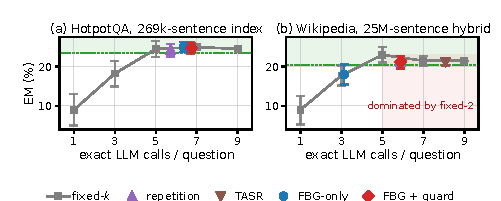
\includegraphics[width=\columnwidth]{figures/fig_frontier_main.pdf}
  \caption{Accuracy versus exact LLM calls in the primary HotpotQA and
  Wikipedia 25M cells. Shading marks the 1-EM admissible band and the fixed-2
  domination region.}
  \label{fig:frontier}
  \Description{Two scatter plots of exact-match accuracy against exact LLM
  calls per question for fixed budgets, answer repetition, TASR, and learned
  stopping policies. Vertical bars show paired 95 percent intervals against
  the full-budget policy. A green band spans accuracies within 1 exact-match
  point of the full budget. In the right panel a red block covers costs at or
  above the fixed-2 budget with accuracy at or below it.}
\end{figure}

\paragraph{Full-budget savings overstate adaptive value.}
On the nine-backbone HotpotQA panel with call accounting, FBG-only removes 27 to
57\% of searches relative to the full budget. Its paired EM differences range
from $-2.1$ to $+2.0$ points, and seven of nine intervals contain zero. The
stronger point-frontier comparison yields a different conclusion. Across the
core 26 cells, FBG-only is dominated in 10 cells, lies on the frontier
without improving $B^\star$ in 13, and improves $B^\star$ in 3. Guarded FBG is
dominated in 15 of 26 cells, is frontier-only in 6, and improves $B^\star$ in
5. Thus it fails to strictly improve the selected fixed budget in 21 of 26
cells. Table~\ref{tab:decision-matrix} reports the complete matrix. Its first
block contains 12 call-only cells, while the final block contains 14 fully
instrumented cells. In the table, C denotes exact LLM calls, $\Delta$ compares
a learned policy with the full budget, and Cat. gives its D, F, or I point
category. These categories prevent a cheap but inaccurate point from being
described as a tie. Cert. gives the SGR outcome. NA marks unavailable
raw features and `refuse' zero certificate coverage.

\begin{table*}[t]
\caption{Complete FBG point audit across 12 call-only and 14 fully instrumented
core cells.}
\label{tab:decision-matrix}
\scriptsize
\setlength{\tabcolsep}{2.6pt}
\rowcolors{3}{}{rowshade}
\begin{tabular}{l r r r r r l c r l c l}
\toprule
\hiderowcolors
& & Full & $B^{\star}$ & Rep. & \multicolumn{3}{c}{FBG-only} &
\multicolumn{3}{c}{Guarded FBG} & \\
\cmidrule(lr){6-8}\cmidrule(lr){9-11}
Cell & $n$ & EM & EM/C\,($B^{\star}$) & EM/C & EM/C & $\Delta$\,[CI] & Cat. &
EM/C & $\Delta$\,[CI] & Cat. & Cert. \\
\midrule
\showrowcolors
HotpotQA / Haiku 4.5 & 140 & 52.1 & 52.1/5.0\,(2) & 50.0/5.47 & 50.7/4.76 & -1.4\,[-5.0,2.1] & F & 51.4/5.71 & -0.7\,[-3.6,1.4] & D & NA \\
HotpotQA / Sonnet 4.5 & 140 & 52.1 & 52.1/7.0\,(3) & 52.9/5.93 & 53.6/6.70 & +1.4\,[0.0,3.6] & I & 53.6/6.77 & +1.4\,[0.0,3.6] & I & NA \\
HotpotQA / GPT-oss-120B & 140 & 57.1 & 59.3/5.0\,(2) & 55.0/4.69 & 55.7/5.97 & -1.4\,[-4.3,1.4] & D & 55.7/6.19 & -1.4\,[-4.3,1.4] & D & NA \\
HotpotQA / Nova Lite & 140 & 54.3 & 54.3/7.0\,(3) & 54.3/5.04 & 52.9/6.87 & -1.4\,[-3.6,0.0] & D & 53.6/6.96 & -0.7\,[-2.1,0.0] & D & NA \\
HotpotQA / Qwen2.5-3B & 140 & 38.6 & 40.0/7.0\,(3) & 39.3/5.87 & 39.3/6.11 & +0.7\,[-3.6,5.0] & D & 40.0/6.73 & +1.4\,[-2.1,5.0] & I & NA \\
HotpotQA / Llama-3.2-3B & 140 & 39.3 & 37.9/5.0\,(2) & 37.9/5.39 & 37.9/5.43 & -1.4\,[-6.4,3.6] & D & 39.3/6.31 & +0.0\,[-4.3,4.3] & F & NA \\
HotpotQA / Command-R-35B & 100 & 51.0 & 52.0/7.0\,(3) & 54.0/5.06 & 53.0/6.76 & +2.0\,[0.0,5.0] & D & 53.0/6.78 & +2.0\,[0.0,5.0] & D & NA \\
HotpotQA / Kimi K2.5 & 140 & 59.3 & 59.3/5.0\,(2) & 56.4/4.67 & 57.9/4.94 & -1.4\,[-5.0,1.4] & F & 57.9/5.31 & -1.4\,[-5.0,1.4] & D & NA \\
HotpotQA / MiniMax M2.5 & 140 & 55.7 & 55.7/9.0\,(4) & 45.0/4.20 & 53.6/4.41 & -2.1\,[-7.1,2.9] & F & 53.6/5.53 & -2.1\,[-6.4,2.1] & F & NA \\
2Wiki / Qwen2.5-3B & 140 & 28.6 & 30.7/7.0\,(3) & 29.3/5.70 & 28.6/6.20 & +0.0\,[-2.9,2.9] & D & 29.3/6.87 & +0.7\,[-1.4,2.9] & D & NA \\
MuSiQue / Qwen2.5-3B & 140 & 13.6 & 12.9/5.0\,(2) & 12.9/6.27 & 12.1/5.09 & -1.4\,[-4.3,1.4] & D & 13.6/6.39 & +0.0\,[0.0,0.0] & F & NA \\
MuSiQue / Llama-3.2-3B & 100 & 18.0 & 18.0/7.0\,(3) & 17.0/5.86 & 16.0/5.86 & -2.0\,[-7.0,3.0] & D & 18.0/6.88 & +0.0\,[-3.0,3.0] & I & NA \\
\midrule
Corpus (seed 7, q-sample A) & 400 & 24.5 & 25.0/7.0\,(3) & 24.2/5.72 & 25.0/6.35 & +0.5\,[-0.8,1.8] & I & 24.8/6.75 & +0.2\,[-0.8,1.5] & F & refuse \\
Corpus (seed 11, q-sample A) & 400 & 25.0 & 25.2/7.0\,(3) & 25.0/5.70 & 25.2/5.74 & +0.2\,[-2.0,2.5] & D & 25.2/6.50 & +0.2\,[-1.0,1.5] & D & refuse \\
Corpus (seed 19, q-sample A) & 400 & 26.0 & 26.0/7.0\,(3) & 25.5/5.71 & 25.2/6.38 & -0.8\,[-2.0,0.5] & D & 25.5/6.67 & -0.5\,[-1.5,0.5] & D & refuse \\
Corpus (seed 7, q-sample B) & 400 & 31.2 & 31.2/9.0\,(4) & 27.8/5.75 & 29.5/6.62 & -1.8\,[-3.5,-0.2] & F & 29.2/6.71 & -2.0\,[-3.5,-0.5] & F & refuse \\
Corpus (seed 7, q-sample C) & 400 & 26.5 & 24.8/7.0\,(3) & 23.2/5.90 & 13.5/2.67 & -13.0\,[-17.0,-9.2] & F & 23.2/5.90 & -3.2\,[-5.2,-1.2] & F & refuse \\
Corpus (seed 7, q-sample D) & 400 & 25.5 & 25.5/9.0\,(4) & 26.5/5.88 & 26.2/5.42 & +0.8\,[-1.5,3.0] & I & 27.0/6.36 & +1.5\,[0.0,3.0] & I & refuse \\
Corpus (seed 7, q-sample E) & 400 & 34.2 & 34.2/9.0\,(4) & 32.0/5.71 & 33.2/7.51 & -1.0\,[-2.2,0.0] & F & 34.2/7.75 & +0.0\,[-0.8,0.8] & I & refuse \\
2Wiki corpus (seed 7, draw 1) & 400 & 23.2 & 24.2/7.0\,(3) & 23.5/5.50 & 20.2/3.11 & -3.0\,[-6.2,0.2] & F & 23.5/5.50 & +0.2\,[-2.0,2.5] & D & refuse \\
2Wiki corpus (seed 7, draw 2) & 400 & 25.2 & 25.2/9.0\,(4) & 23.2/5.51 & 19.0/3.83 & -6.2\,[-9.2,-3.5] & F & 23.5/5.59 & -1.8\,[-3.8,0.0] & D & refuse \\
2Wiki corpus (seed 7, draw 3) & 400 & 25.5 & 26.2/5.0\,(2) & 25.2/5.61 & 24.2/3.12 & -1.2\,[-4.8,2.2] & F & 25.8/5.66 & +0.2\,[-1.8,2.2] & D & refuse \\
MuSiQue corpus (seed 7, draw 1) & 400 & 9.2 & 7.2/7.0\,(3) & 7.5/6.53 & 3.8/3.02 & -5.5\,[-8.2,-3.0] & F & 7.5/6.54 & -1.8\,[-3.2,-0.5] & D & refuse \\
MuSiQue corpus (seed 7, draw 2) & 400 & 10.2 & 10.2/9.0\,(4) & 9.2/6.45 & 2.5/1.44 & -7.8\,[-10.5,-5.2] & F & 9.2/6.50 & -1.0\,[-2.5,0.2] & D & refuse \\
MuSiQue corpus (seed 7, draw 3) & 400 & 12.0 & 10.8/7.0\,(3) & 10.8/6.42 & 0.2/1.00 & -11.8\,[-15.0,-8.8] & F & 10.8/6.42 & -1.2\,[-2.5,-0.2] & D & refuse \\
Wikipedia 25M hybrid & 400 & 21.5 & 23.0/5.0\,(2) & 21.2/5.88 & 18.0/3.13 & -3.5\,[-6.0,-1.0] & F & 21.2/5.89 & -0.2\,[-2.0,1.2] & D & refuse \\

\bottomrule
\end{tabular}
\end{table*}

Figure~\ref{fig:frontier} illustrates why the comparator matters. In the
primary HotpotQA cell, guarded FBG reaches 24.75 EM at 6.75 calls versus 24.50
at 9.00 for the full budget. FBG-only is cheaper and has slightly higher point
accuracy than the guard. Fixed-2, however, remains competitive on the same
frontier. In the Wikipedia boundary cell, fixed-2 reaches 23.00 EM at 5.00
calls and strictly dominates guarded FBG at 21.25 EM and 5.90 calls. The
learned policy saves work relative to full search without creating a better
deployment option.

The oracle separates available headroom from signal identification. We use a
nondeployable hindsight rule that reads every
prefix grade, stops at the first correct prefix, and charges the full budget
when no prefix is correct. Table~\ref{tab:oracle-ceiling} reports this ceiling
for the 14 fully instrumented core cells, with cell labels from
Table~\ref{tab:decision-matrix}.

\begin{table}[t]
\caption{Hindsight-oracle ceiling for fourteen fully instrumented cells. Never-correct
questions incur the full budget.}
\label{tab:oracle-ceiling}
\scriptsize
\setlength{\tabcolsep}{3.1pt}
\rowcolors{2}{rowshade}{}
\begin{tabular}{@{}lrrrrr@{}}
\toprule
\hiderowcolors
Cell & Full EM & Oracle EM & Gain & Searches & Calls \\
\midrule
\showrowcolors
HotpotQA A, seed 7 & 24.50 & 29.50 & +5.00 & 3.14 & 7.28 \\
HotpotQA A, seed 11 & 25.00 & 30.25 & +5.25 & 3.12 & 7.24 \\
HotpotQA A, seed 19 & 26.00 & 30.25 & +4.25 & 3.13 & 7.25 \\
HotpotQA sample B & 31.25 & 37.00 & +5.75 & 3.00 & 7.00 \\
HotpotQA sample C & 26.50 & 30.25 & +3.75 & 3.23 & 7.46 \\
HotpotQA sample D & 25.50 & 32.25 & +6.75 & 3.12 & 7.24 \\
HotpotQA sample E & 34.25 & 39.00 & +4.75 & 2.94 & 6.88 \\
2Wiki draw 1 & 23.25 & 30.25 & +7.00 & 3.12 & 7.23 \\
2Wiki draw 2 & 25.25 & 31.25 & +6.00 & 3.15 & 7.31 \\
2Wiki draw 3 & 25.50 & 33.50 & +8.00 & 3.04 & 7.08 \\
MuSiQue draw 1 & 9.25 & 11.25 & +2.00 & 3.78 & 8.55 \\
MuSiQue draw 2 & 10.25 & 12.50 & +2.25 & 3.71 & 8.43 \\
MuSiQue draw 3 & 12.00 & 13.75 & +1.75 & 3.69 & 8.39 \\
Wikipedia 25M & 21.50 & 26.75 & +5.25 & 3.19 & 7.38 \\

\bottomrule
\end{tabular}
\end{table}

The oracle dominates full search in all fourteen cells, with gains from
$+1.75$ to $+8.00$~EM and a mean gain of $+4.84$. In the primary cell, it
reaches $29.50$~EM at $3.14$ searches and $7.28$ calls, compared with
$24.50$~EM at four searches and nine calls for full search. Guarded FBG
reaches $24.75$~EM in that cell. The oracle therefore establishes measurable
stopping headroom, while the learned gap localizes the bottleneck to reliable
identification. It remains a diagnostic upper bound rather than a deployable
policy.

We next compare the signal families at point and matched cost. In
Table~\ref{tab:whowins}, Scope gives point and cost cell counts, $\Delta$ range
gives the cellwise extremes against the equal-call hull, and Cell $+/-$ counts
marginally resolved positive and negative intervals. Bonf. and Max-t count
corrected positives, and NA marks unretained vectors.

\begin{table}[t]
\caption{Cross-signal frontier and matched-cost summary over the principal
18-cell family.}
\label{tab:whowins}
\scriptsize
\setlength{\tabcolsep}{2.2pt}
\rowcolors{3}{rowshade}{}
\begin{tabular}{@{}lrrrrrr@{}}
\toprule
\hiderowcolors
Signal & Scope & D/F/I & $\Delta$ range & Cell $+/-$ & Bonf. & Max-t \\
\midrule
\showrowcolors
FBG-only & 18/18 & 2/14/2 & $-2.38,1.86$ & 0/2 & 0 & 0 \\
Guarded FBG & 18/18 & 11/5/2 & $-1.89,0.85$ & 0/2 & 0 & 0 \\
Stop classifier & 18/18 & 1/15/2 & $-2.40,2.61$ & 3/1 & 1 & 0 \\
Error-head gate & 18/18 & 9/9/0 & $-1.50,0.70$ & 1/0 & 1 & 0 \\
Gold-support sufficiency & 18/18 & 8/8/2 & $-2.00,0.47$ & 0/1 & NA & NA \\
Full TASR & 12/12 & 5/6/1 & $-1.75,0.53$ & 0/0 & 0 & 0 \\
Stop-RAG & 14/14 & 9/4/1 & $-3.00,0.50$ & 0/3 & 0 & 0 \\

\bottomrule
\end{tabular}
\end{table}

\paragraph{Cellwise gains do not survive family-wise inference.}
Policy-specific eligibility explains why TASR and Stop-RAG do not cover all 18
cells. Neither FBG policy has a positive cellwise equal-call interval,
and each has two negative intervals. The binary future-improvement classifier
has three positive intervals and one negative interval. Its largest gain is
$+0.11$ EM with Bonferroni interval $[+0.03,+0.19]$. The error-head gate has
one positive estimate of $+0.14$ EM with Bonferroni interval
$[+0.02,+0.33]$. Neither remains positive under its max-t simultaneous band.
Bonferroni uses percentile intervals, whereas max-t uses studentized
simultaneous bands, so their resolved sets need not be nested. The two
corrected gains remain below $0.2$ EM and are operationally small.
Gold-support sufficiency lacks the per-question vectors required for a max-t
band, so we mark that analysis NA rather than treating it as zero. We thus
make no family-wise directional claim.

We repeat the hull comparison at matched calls, input tokens, and wall time.
Across the 14 fully instrumented cells, guarded FBG differs from the matched
hull by $-0.59$, $-0.64$, and $-0.60$ EM, with no positive FBG interval in
any currency. Under an answer-once ledger, guarded FBG is dominated in 17 of
18 cells and repetition in all 18. The repetition baseline is therefore useful
only when prefix answers are already generated.

\paragraph{Precision of the matched-cost comparisons.}
Across the 18-cell family, the saved cellwise 95\% equal-call intervals have
median width 2.75 EM points for guarded FBG (range 0.06 to 3.75) and 2.98 for
FBG-only (range 0.00 to 8.48). These intervals condition on the fitted
policies and matching hull. A zero-width contrast can arise from identical
recorded outcomes and does not imply zero uncertainty in a new population.
The 1.39-EM power calculation in the setup concerns full search and must not be
transferred to this comparator. In particular, 44 answer disagreements among
2,000 question-draw records do not resolve small gains against a different
matched-cost reference. Unresolved intervals establish neither equivalence
nor absence of a useful effect.
\paragraph{Matched and transplanted alternatives.}
Within the 14 fully instrumented core cells, FBG-only is nondominated in 11
of 14, fixed-2 in 12, and the binary future-improvement classifier in 13. On
the wider 18-cell family, Stop-RAG is dominated in 9 of 14 eligible cells and
has three negative but no positive equal-call intervals. Full TASR is
nondominated in 7 of 12 eligible cells. An NLI-augmented FBG variant is the
cheapest policy within 1 EM of full search in only 1 of 14 cells. The
supplement reports the transplanted systems and verifier-inspired substitutes,
whose different generation designs support contextual rather than matched
claims.

\Needspace{12\baselineskip}
\subsection{RQ2: Does the decision persist?}
\label{sec:replication}

\paragraph{Question resampling changes the endpoint decision.}
On 400 untouched HotpotQA questions, guarded FBG reaches 24.75 EM versus
24.50 for the full budget. The paired difference is $+0.25$ with a 95\%
interval of $[-0.75,1.50]$ and a one-sided lower bound of $-0.75$. Calls fall
from 9.00 to 6.75, input tokens fall by 30.7\%, output tokens by 27.1\%, and
wall time by 23.8\%. The endpoint therefore passes the declared 3-EM
non-inferiority and call-reduction rule. The two-sided interval contains zero,
so the matched-cost and replication analyses determine the stronger claim.

\begin{figure}[t]
  \centering
  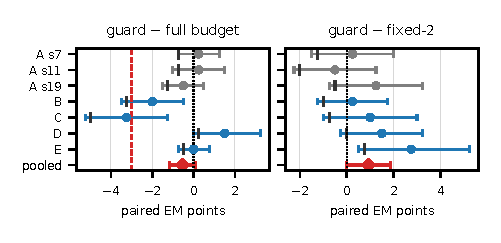
\includegraphics[width=\columnwidth]{figures/fig_samples_main.pdf}
  \caption{Guarded FBG minus full search or two fixed searches. Grey rows rerun
  HotpotQA sample A with new seeds, and blue rows are new question samples.}
  \label{fig:samples}
  \Description{Forest plot of paired exact-match differences between guarded
  FBG and full search or two fixed searches. Each row is one run. Bars show 95 percent
  intervals, ticks show one-sided lower bounds, and a dashed line marks the
  negative three point margin.}
\end{figure}

Figure~\ref{fig:samples} separates decoding and population variation. With the
same 400 questions, decoding seeds 7, 11, and 19 give guarded differences of
$+0.25$, $+0.25$, and $-0.50$ EM. All pass the predeclared rule. Four new
question draws give $-2.00$, $-3.25$, $+1.50$, and $0.00$ EM. Their one-sided
lower bounds are $-3.25$, $-5.00$, $+0.25$, and $-0.50$, so two of four pass
and two fail. Across all five question samples, three of five pass. The two
negative cellwise intervals do not remain directional under the max-t
family-wise band. The draw disagreement is the substantive result because it
overturns the stable decision suggested by same-question decoding reruns.

The draw-level mean is $-0.70$ EM with one-sided lower bound $-2.51$. Pooled
contrasts against full search and fixed-3 are $-0.54$ $[-1.18,0.11]$ and
$-0.32$ $[-1.03,0.37]$ EM, and both contain zero. Contrasts favoring the guard over fixed-2 or repetition use
1.67 and 0.90 more calls. Thus every favorable pooled contrast costs more,
while every equal-cost or lower-cost contrast remains unresolved.

Between-draw contrast variation is larger than the same-question decoding
variation in this small panel. With five question draws and three decoding
seeds, we do not estimate a stable variance decomposition. Descriptively,
$I^2=80\%$ is the share of observed heterogeneity beyond within-draw
uncertainty, while $\tau=1.25$ EM is the estimated between-draw standard
deviation. Neither is a population parameter in this five-draw panel. Only 44
of 2{,}000 questions produce different full-budget and guarded answers, so a
small item set can determine a draw-level decision.

\paragraph{Backbone crosses and Wikipedia-derived datasets.}
Three Claude Haiku 4.5 draws with $n=200$ and one Llama-3.2-3B draw with
$n=400$ all pass the 3-EM margin. Guarded FBG reaches the pooled frontier in
none, and its mean equal-call difference is $+0.14$ EM. Changing the backbone
therefore changes the accuracy level more than the deployment verdict.

On the 25{,}247{,}888-sentence FEVER Wikipedia index, guarded FBG has paired
difference $-0.25$ EM with interval $[-2.00,1.25]$ and lowers calls from 9.00
to 5.90. Fixed-2 still dominates it. Three 2Wiki draws lower calls to between
5.5 and 5.7, but fixed-2 dominates the guard in every draw. On three MuSiQue
draws, answer repetition or fixed-2 also dominates the guard. The repeated
domination extends the result beyond one Wikipedia-derived benchmark. We
interpret these cells as related environments because they share a sparse
retrieval stack and multi-hop task design.

\paragraph{One external news-corpus cell.}
We froze one MultiHopRAG inference-query cell before fitting or test
evaluation. It contains 400 questions over 609 English news articles and uses
Qwen2.5-3B with the same four-search cap. Table~\ref{tab:external-policies}
separates the frozen FBG endpoint from three exploratory signal policies. Each
gain compares a policy to the randomized simple hull at equal
mean calls.

\begin{table}[H]
\caption{External news-cell policies at equal calls to the simple-policy hull.}
\label{tab:external-policies}
\footnotesize
\setlength{\tabcolsep}{8.4pt}
\rowcolors{2}{rowshade}{}
\begin{tabular}{@{}lrrrl@{}}
\toprule
\hiderowcolors
\tabhead \textbf{Policy} & \textbf{EM} & \textbf{Calls} & \textbf{Gain vs.\ simple} & \textbf{95\% CI} \\
\midrule
\showrowcolors
FBG-only & 73.00 & 7.27 & $+0.48$ & $[-0.50,1.46]$ \\
Guarded FBG & 73.25 & 7.40 & $+0.71$ & $[-0.07,1.57]$ \\
Stop classifier & 70.50 & 4.35 & $+2.10$ & $[0.12,4.10]$ \\
Error-head gate & 73.75 & 7.65 & $+1.18$ & $[0.41,2.06]$ \\

\bottomrule
\end{tabular}
\end{table}

Guarded FBG reaches 73.25 EM at 7.40 calls, compared with 72.75 EM at 9.00
calls for full search. It passes the declared endpoint, but the
matched-cost advantage remains unresolved. The binary future-improvement and
error-head intervals are positive, yet both policies are exploratory and come
from one question draw.
The cell therefore shows that the signal choice can change a boundary result.
As a single draw with a per-cell refitted head, it does not establish
cross-domain controller transfer.


\subsection{RQ3: Which stopping signal is informative?}

\paragraph{Current error provides the stronger risk ordering.}
At each selected stop, we rank questions by predicted risk. We define
risk-coverage area as mean stopped-answer error over coverage fractions from
0.05 to 1.00, with lower values preferred, and compare it with 20 random
orderings. We also report expected calibration error (ECE) and area under the
receiver operating characteristic curve (AUROC). Table~\ref{tab:signal-diagnostics}
shows that our current-error head improves on random in every cell, while FBG
does so in 7 of 18. This ordering gap explains how FBG can save calls without
assigning extra search to the questions that benefit from it.

\begin{table}[t]
\caption{Signal and trajectory diagnostics for RQ3. Test labels evaluate the
frozen outputs and never select a policy.}
\label{tab:signal-diagnostics}
\footnotesize
\setlength{\tabcolsep}{3pt}
\rowcolors{2}{rowshade}{}
\begin{tabular}{@{}p{0.31\columnwidth}p{0.17\columnwidth}p{0.43\columnwidth}@{}}
\toprule
\hiderowcolors
Diagnostic & Scope & Measured result \\
\midrule
\showrowcolors
FBG risk ordering & 18 cells & Better than random in 7 cells \\
Error-head ordering & 18 cells & Better than random in all 18 cells \\
Error calibration & 18 cells & Test-prefix ECE 0.019 to 0.087, median 0.043 \\
Gold-support coverage & 18 cells & Cross-fitted AUROC 0.652 to 0.946 \\
Late answer reversals & 1{,}220 pairs & 79 harmful and 14 helpful \\
Rerolled futures & 300 stops & Beat logged best in 10.0\%, changed correctness in 5.7\% \\
\bottomrule
\end{tabular}
\end{table}

\paragraph{Predictive discrimination does not guarantee policy utility.}
Our same-feature gold-support classifier separates evidence-coverage states
with AUROC from 0.652 to 0.946, yet its D/F/I tally is 8/8/2 with no cellwise
equal-call win. The future-improvement classifier is dominated in only one
cell, but its three positive intervals disappear under max-t correction.
State discrimination alone therefore does not establish policy utility.

The current-error target asks whether the present answer is wrong, whereas
FBG must predict a useful later reversal from incomplete prefix information.
The former can rank risk without identifying whether another search will
repair it. Threshold choice and population shift then add two further gaps
between ranking and policy value. These mechanisms are consistent with the
observed diagnostics, not a causal decomposition of the oracle gap.
\paragraph{Late retrieval creates headroom that FBG only partly captures.}
Late retrieval produces 79 harmful and 14 helpful reversals, with a 95\% ratio
interval of 3.2 to 11.1 and $p<10^{-3}$. Guarded FBG realizes 24 beneficial
and 32 harmful flips. FBG captures only part of this stopping headroom.

\paragraph{Refitting and rerolling localize the instability.}
Held-out-prefix FBG correlations range from 0.26 to 0.60 and absolute errors
from 0.12 to 0.19. We therefore repeat fitting and both learned and simple
selection in 400 chain-bootstrap resamples per run. This analysis conditions
on logged questions, retrieval, preprocessing, and decoding, so it isolates
fit-and-selection instability.

\begin{figure}[t]
  \centering
  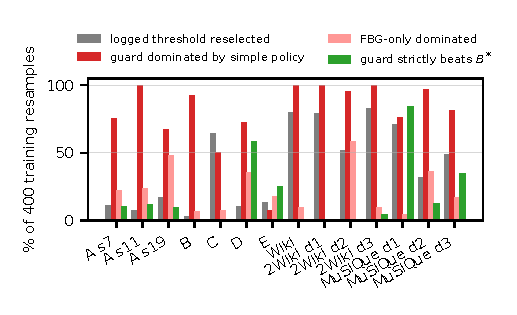
\includegraphics[width=0.88\columnwidth]{figures/fig_nested.pdf}
  \caption{Nested refit and reselection across 400 training-chain resamples per
  fully instrumented run.}
  \label{fig:nested}
  \Description{Grouped bars show the shares of bootstrap replications that
  retain the logged threshold, are dominated by a reselected simple policy,
  or beat the reselected fixed budget.}
\end{figure}

Figure~\ref{fig:nested} makes the selection instability operational. The logged
threshold is reselected in only 3 to 17\% of resamples on six of seven HotpotQA
conditions. A simple policy dominates in 51 to 100\% of resamples in seven of
eight reported runs.

Two rerolled continuations per primary-cell stop beat the logged best in 10.0\%
of cases and change correctness in 5.7\%. These are reachable gains outside the logged path.

The original clipped target variants move mean guarded EM by at most
0.2 points. The logged guarded policies have D/F/I counts 9/3/2 across the
14 instrumented cells. Refitting the full feature set and reselecting the
threshold gives 11/2/1, whereas removing step, evidence-count, and stability
features gives 11/1/2. These are different fitted policies, not conflicting
tallies of the logged matrix: only 8 of 14 refits recover the logged threshold.
Across 154 protocol variants, simple policies dominate 114 and the guard
Pareto-improves $B^\star$ in 17. These probes delimit sensitivity within the
logged regime rather than exclude gains from other designs.

Across 1{,}400 training-size refits, moving from 30 to 90 episodes lowers
domination by 6.1 points and raises mean EM by 0.14, nonmonotonically.
Pooling training chains from same-environment cells (up to 421 episodes) or
all 14 cells (up to 959), excluding target test questions, cuts guarded
domination from 11 to 8 and 9 cells and FBG-only domination from 10 to 4 and 6.
Mean matched-cost gaps remain $-0.22$ to $-0.53$ EM. Of 56 paired intervals,
1 favors the learned policy and 6 the mixture. More data moves points toward
the frontier without resolving a gain (supplement).

\paragraph{Retrospective signed-target and deterministic-control checks.}
On the same 14 cells, a signed best-future target uses the original features,
five-fold training-chain cross-fitting, and threshold grid. The guarded
signed refit has D/F/I counts 11/3/0, compared with 11/2/1 for a freshly
refitted clipped target. Mean EM changes from 22.13 to 22.05, while mean calls
fall from 6.44 to 6.26, isolating clipping, not horizon. We also select a deterministic evidence-growth rule on training chains:
after at least one search, stop when newly retained units are at most a
threshold in $\{0,1,2,3\}$. Adding this rule to the simple family gives
D/F/I counts 11/2/1 for logged guarded FBG and 3/9/2 for FBG-only.
Across calls, tokens, and a wall-time proxy, mean matched-cost gaps are
negative and all 84 conditional simultaneous bands include zero (supplement).
These exploratory checks preserve the frozen 26-cell analysis.
A fresh eight-search Haiku 4.5 check uses 120 training and 200 test questions.
FBG-only reaches 55.5 EM at 8.19 calls, but all 12 conditional simultaneous
matched-cost bands across horizons four and eight include zero (supplement).

\subsection{RQ4: Can we certify stopped answers?}

For each of 14 fully instrumented cells, we reserve 30 of 120 development
episodes, fit the error scorer on 90, and evaluate one guarded-policy stop per
calibration and test episode. Corrected SGR accepts none of the 84 cell and
target-risk pairs over six $\alpha$ values, so Table~\ref{tab:certificate-coverage}
reports zero coverage. This fail-closed result withholds an unsupported
reliability claim.

{\setlength{\intextsep}{6pt}
\begin{table}[t]
\caption{Deployment-matched SGR results for RQ4 with 30 calibration episodes
per cell.}
\label{tab:certificate-coverage}
\footnotesize
\setlength{\tabcolsep}{3pt}
\rowcolors{2}{rowshade}{}
\begin{tabularx}{\columnwidth}{@{}lRRR@{}}
\toprule
\hiderowcolors
\tabhead \textbf{Population} & \textbf{Cells} & \textbf{Accepted pairs} & \textbf{Test coverage} \\
\midrule
\showrowcolors
HotpotQA corpus & 7 & 0/42 & 0\% \\
2WikiMultihopQA & 3 & 0/18 & 0\% \\
MuSiQue & 3 & 0/18 & 0\% \\
Wikipedia 25M & 1 & 0/6 & 0\% \\
\midrule
\hiderowcolors
\textbf{All} & \textbf{14} & \textbf{0/84} & \textbf{0\%} \\
\bottomrule
\end{tabularx}
\end{table}
}

We restrict the claim to deployment-matched prefix features. The supplement
quarantines score-mismatched call-only diagnostics.


\section{Scope and Practical Guidance}
\label{sec:limitations}

The core audit covers nine-feature heads trained on 30 to 90 per-cell
(at most 959 pooled) trajectories in four-search replay over static English
corpora. The supplement adds a fresh eight-search Haiku 4.5 check. Other
retrievers, languages, hidden states, and joint query control require new
frontiers. Per-cell refitting tests recurrence, not frozen transfer. FBG
labels one realized continuation rather than counterfactual actions.

Counts summarize heterogeneous cells. Nested resampling conditions on logged
trajectories and decoding, whereas independent draws test population variation.
Low-EM cells assess controller differences, not answer quality. Historical
ledgers omit lifecycle, invoice, energy, retry, and failure costs. Repetition
requires prefix answers, and other execution schedules need separate frontiers.

For transfer, declare state and costs, select references on development data,
freeze policies, and evaluate independent questions with paired and simultaneous
intervals. Keep stopping replay separate from jointly learned query control.
Fresh same-population policy training beyond 90 chains remains untested.
Code and outputs: \url{https://github.com/lexuanbach/wsdm2027-learned-stopping-audit}.

\section{Conclusion}
\label{sec:conclusion}
The oracle exposes stopping headroom, but the evaluated guarded FBG has no resolved
improvement over tuned simple controls at matched cost. Independent question draws
also overturn same-question stability. Current-error estimates rank risk more
reliably, yet ranking alone does not establish policy utility. In this regime,
the selected fixed budget remains our default until a learned controller
passes an independent, multiplicity-aware frontier test.

\phantomsection\label{body:end}
\clearpage
\section*{Ethical Considerations}

\paragraph{Errors from premature stopping.}
A controller can reduce resource use while withholding evidence that would
correct an answer. This risk may be concentrated on topics that are rare in
the development data, including questions involving underrepresented regions,
languages, or communities. We therefore evaluate quality and cost jointly and
recommend deployment only after an independent, task-specific frontier test.
The current evidence is English-only and does not support conclusions about
multilingual equity.

\paragraph{Limits of certification.}
The certificate in Proposition~\ref{prop:conformal} is marginal under an
independent and identically distributed calibration and test assumption. It
does not bound risk for an individual question or subgroup and must not be
presented as a per-answer probability of correctness. Corrected SGR refuses
every evaluated target. A deployment should expose that absence rather than
silently treating an uncertified answer as safe. It should also recalibrate by
task family and monitor subgroup risk after distribution shift.

\paragraph{Resource claims and operational telemetry.}
Our fully instrumented runs measure LLM calls, input and output tokens, and wall time. We do
not measure energy, invoice cost, or the marginal environmental effect of a
provider call. The execution code does not retain timeout and retry failure
codes, so we cannot report a failure rate. We make these omissions explicit to
avoid converting lower measured calls into an unsupported energy, monetary,
or reliability claim. The small stopping predictors train on CPU and the base
backbones remain frozen.

\paragraph{Data, access, and dual use.}
HotpotQA, 2WikiMultihopQA, MuSiQue, FEVER, and MultiHopRAG are public research
datasets used under their respective terms. The evaluated material includes
Wikipedia-derived text and one English news snapshot. We use no private user
or production data and access no live websites. The artifact's trajectories may
repeat public biographical or news facts and should be handled under the
source datasets' licenses. The same stopping machinery could be tuned for
cheap but unreliable answering. Publishing the selection and calibration
failures makes that tradeoff inspectable rather than endorsing such use.


\bibliographystyle{ACM-Reference-Format}
\bibliography{references}

\end{document}
